\documentclass[11pt,a4paper]{article}
\usepackage[top=2.2cm,bottom=2.2cm,left=2.5cm,right=2.3cm]{geometry}
\usepackage[utf8]{inputenc}
\usepackage[T5]{fontenc}
\usepackage{lmodern}
\usepackage{graphicx,float,booktabs,array,xcolor,listings,caption,subcaption,fancyhdr,tikz,enumitem,tcolorbox}
\usetikzlibrary{arrows.meta,positioning,shapes.geometric,fit,backgrounds,calc}
\usepackage[colorlinks=true,linkcolor=blue!50!black,urlcolor=blue!60!black]{hyperref}
\setlength{\parskip}{3pt}\setlength{\textfloatsep}{8pt}\setlength{\parindent}{0pt}
\linespread{1.03}
\captionsetup{font=small,labelfont=bf}
\pagestyle{fancy}\fancyhf{}
\fancyhead[L]{\small Báo cáo thực hành -- TurtleBot 4: Localization, Nav2 và YOLO}
\fancyfoot[C]{\thepage}
\definecolor{codebg}{gray}{0.96}
\lstset{basicstyle=\ttfamily\scriptsize,backgroundcolor=\color{codebg},frame=single,rulecolor=\color{black!25},
  breaklines=true,columns=fullflexible,keepspaces=true,showstringspaces=false,
  keywordstyle=\color{blue!60!black}\bfseries,commentstyle=\color{green!40!black}\itshape,
  stringstyle=\color{red!55!black},language=Python,numbers=left,numberstyle=\tiny\color{gray},xleftmargin=1.6em}
\newcommand{\rospkg}[1]{\texttt{#1}}
\newcommand{\figw}[2]{\includegraphics[width=#1\linewidth]{figures/#2}}

\begin{document}

%================== TRANG BÌA ==================
\begin{titlepage}
\thispagestyle{empty}
\centering
{\large\bfseries TRƯỜNG / KHOA .......................................\par}
\vspace{0.6cm}
{\large Môn học: Robot tự hành / Lập trình ROS 2\par}
\vspace{1.6cm}
{\huge\bfseries BÁO CÁO BÀI THỰC HÀNH\par}
\vspace{0.6cm}
{\Large Định vị (AMCL), điều hướng tự động bằng Nav2\\ và nhận diện vật thể bằng YOLO\\ trên TurtleBot 4 (Gazebo)\par}
\vspace{1cm}
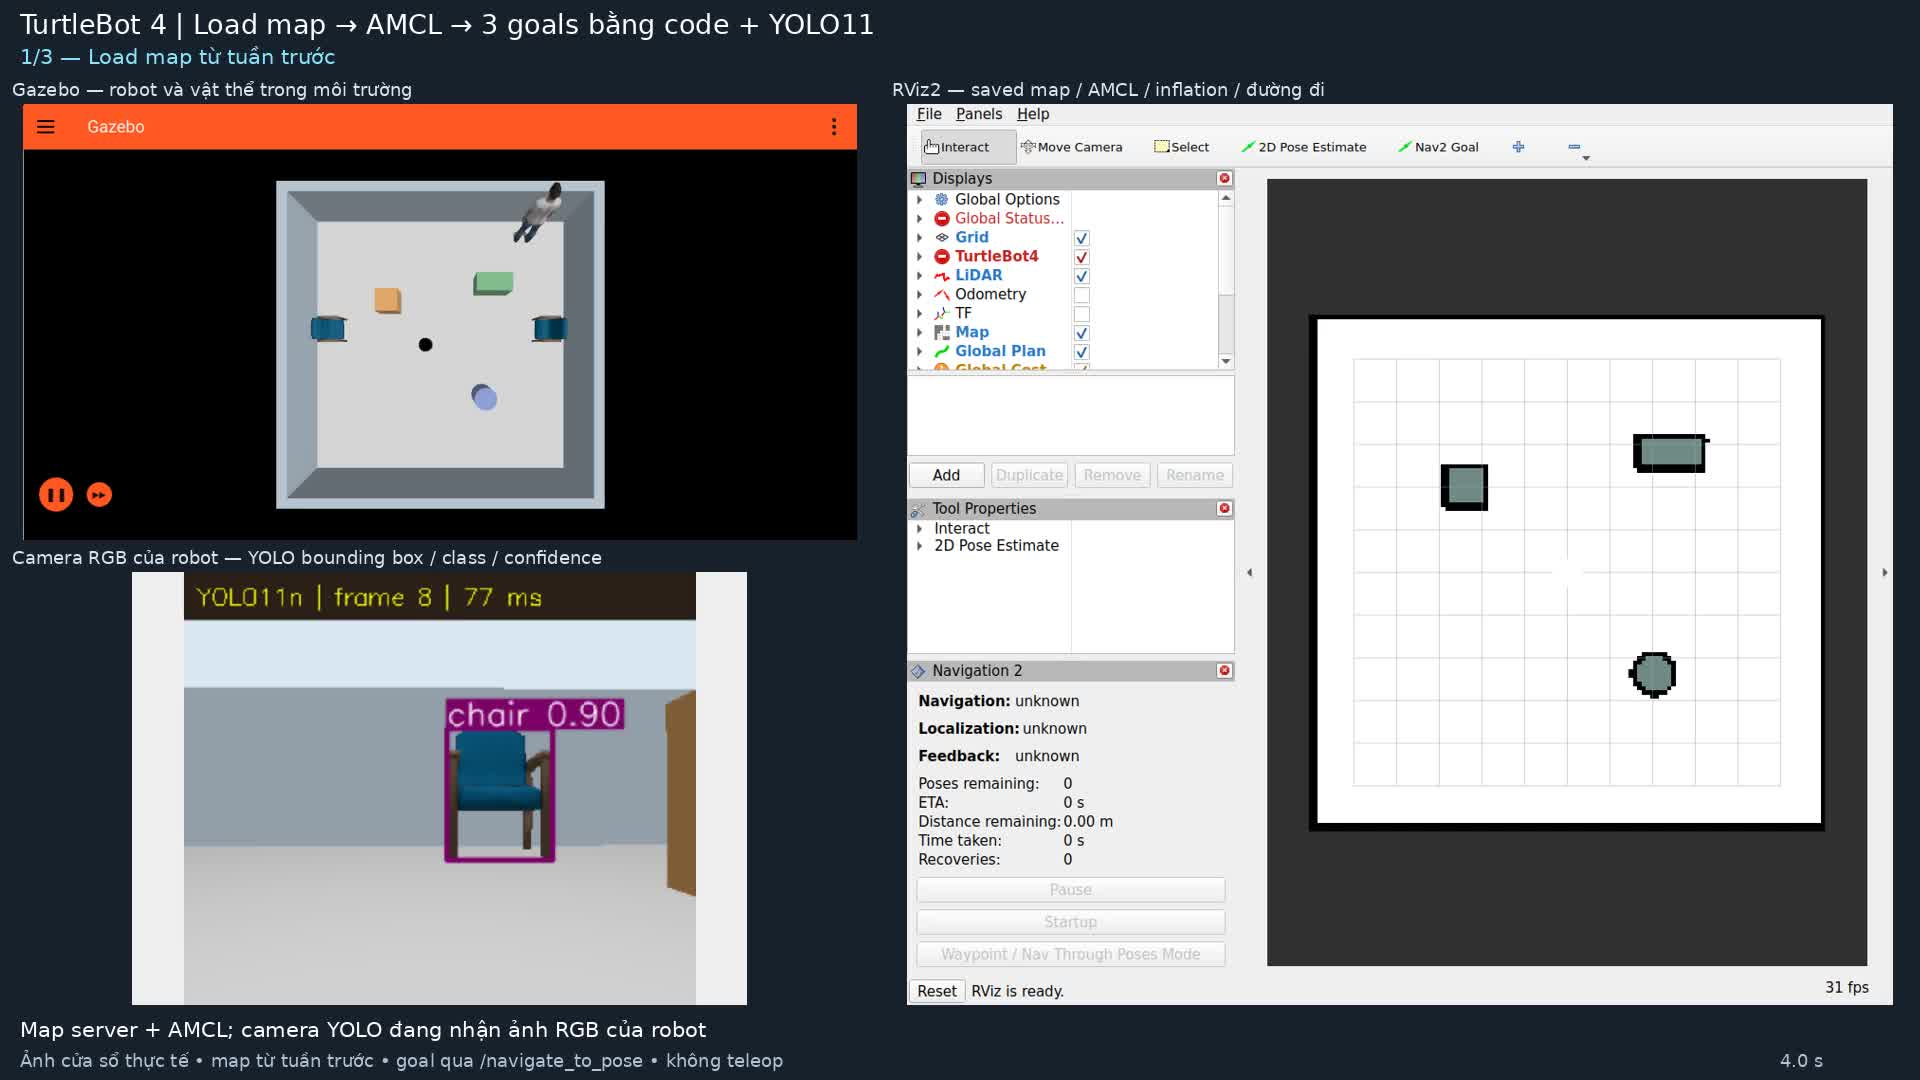
\includegraphics[width=0.7\linewidth]{figures/overview_load.jpg}\par
\vspace{1cm}
\begin{tabular}{rl}
Sinh viên thực hiện: & Trần Thắng \\
Email: & thangtran2792005@gmail.com \\
Nền tảng: & Ubuntu 22.04, ROS 2 Humble, Ignition Gazebo \\
Ngày hoàn thành: & 14/10/2026 \\
\end{tabular}
\vfill
\begin{tabular}{rl}
\textbf{Video demo:} & \href{https://drive.google.com/drive/folders/1LF-GkSyY50TnkUzGGbq_RCvAMGTMZOS7?hl=vi}{Google Drive} \\
\textbf{GitHub:} & \href{https://github.com/TranThang27/UR3_drawing/tree/turtlebot/turtlebot}{github.com/TranThang27/UR3\_drawing (nhánh \texttt{turtlebot})} \\
\end{tabular}
\end{titlepage}

\pagenumbering{arabic}
\tableofcontents
\newpage

%================== 1. GIỚI THIỆU ==================
\section{Giới thiệu và mục tiêu}
Bài thực hành tuần này tái sử dụng bản đồ \texttt{map.yaml}/\texttt{map.pgm} đã xây dựng bằng SLAM Toolbox ở tuần trước để thực hiện ba việc trên robot TurtleBot 4 trong môi trường mô phỏng Gazebo:
\begin{enumerate}[nosep]
  \item \textbf{Localization}: nạp lại bản đồ, chạy AMCL và đặt initial pose sao cho dữ liệu LiDAR \texttt{/scan} trùng khớp với tường trên bản đồ (Phần~1);
  \item \textbf{Navigation tự động bằng code}: một ROS 2 node Python gửi lần lượt ít nhất 3 goal tới action \texttt{/navigate\_to\_pose} của Nav2, không dùng teleop hay chuột đặt goal (Phần~2--3);
  \item \textbf{Object detection}: node thứ hai subscribe ảnh RGB của camera OAK-D, chuyển sang OpenCV bằng \texttt{cv\_bridge}, chạy YOLO11 và hiển thị/publish kết quả song song khi robot di chuyển (Phần~4).
\end{enumerate}
Toàn bộ mã nguồn, bản đồ, cấu hình và hướng dẫn chạy được đưa lên GitHub (nhánh \texttt{turtlebot}); video demo được upload lên Google Drive. Các kết quả (số liệu, ảnh) trong báo cáo được trích từ một lần chạy hoàn chỉnh của chương trình và lưu trong thư mục \texttt{reports/nav\_yolo\_demo\_20261014}.

\paragraph{Tóm tắt kết quả.}
\begin{itemize}[nosep]
  \item Localization đạt: sai lệch vị trí AMCL so với Gazebo ngay sau khi đặt initial pose là $0{,}019$ m và $0{,}93^\circ$ (ngưỡng $0{,}2$ m và $15^\circ$).
  \item Robot đi qua \textbf{3/3 goal} liên tiếp, cả ba trạng thái \texttt{SUCCEEDED}, \textbf{0} lần va chạm (bumper), \textbf{0} lệnh vận tốc thủ công.
  \item YOLO11n xử lý 378 khung hình, phát hiện đúng ghế (độ tin cậy cao nhất $0{,}93$) và người ($0{,}93$) trong khi robot di chuyển.
\end{itemize}

%================== 2. CẤU TRÚC ==================
\section{Cấu trúc chương trình và luồng hoạt động}
\subsection{Cấu trúc thư mục mã nguồn}
Mã nguồn nằm trong thư mục \texttt{turtlebot/} của repository. Chương trình không đóng gói thành \rospkg{ament} package mà dùng \texttt{run.sh} làm điểm vào duy nhất: script source ROS 2 Humble, đặt \texttt{ROS\_DOMAIN\_ID=42}, dùng RMW CycloneDDS rồi gọi launch file hoặc script Python tương ứng.
\begin{lstlisting}[language={},numbers=none]
turtlebot/
|-- run.sh                    # diem vao: ./run.sh {sim|localize|nav2|goals|yolo|yolo-demo|...}
|-- environment.sh            # ROS_DOMAIN_ID, CycloneDDS, overlay cho runtime
|-- launch/
|   |-- simulation.launch.py  # Gazebo (world simple_square) + TurtleBot 4 + RViz2
|   `-- navigation.launch.py  # map_server + AMCL (+ Nav2 neu navigation:=true)
|-- maps/map.yaml, map.pgm    # ban do tuan truoc (121x121 px, 0.05 m/px)
|-- config/goals.yaml         # 3 toa do muc tieu (x, y, yaw) trong frame map
|-- config/*.rviz             # cau hinh RViz2
|-- worlds/simple_square.sdf  # moi truong Gazebo phong 6x6 m
`-- scripts/
    |-- check_navigation.py   # NODE DIEU HUONG: gui Goal1->2->3 qua /navigate_to_pose
    |-- yolo_camera.py        # NODE YOLO: /oakd/rgb/preview/image_raw -> YOLO11
    |-- check_localization.py # dat initial pose + kiem chung AMCL vs Gazebo
    |-- add_demo_objects.py   # them ghe, nguoi vao Gazebo
    |-- run_yolo_demo.py      # chay toan bo quy trinh + quay video
    `-- setup_yolo.py         # cai torch (CPU), ultralytics, trong so yolo11n.pt
\end{lstlisting}

\subsection{Luồng hoạt động tổng thể}
Hình~\ref{fig:arch} mô tả luồng dữ liệu. Gazebo cung cấp \texttt{/scan}, \texttt{/odom} và ảnh camera qua \texttt{ros\_gz\_bridge}. AMCL kết hợp bản đồ do \texttt{map\_server} phát với \texttt{/scan} và odometry để xuất phép biến đổi \texttt{map}$\to$\texttt{odom}. Nav2 dùng TF này để lập kế hoạch toàn cục/cục bộ và xuất \texttt{/cmd\_vel}. Node điều hướng chỉ làm \emph{action client}, còn node YOLO độc lập hoàn toàn với Nav2 và chỉ đọc camera nên hai node chạy song song.

\begin{figure}[htbp]
\centering
\resizebox{\linewidth}{!}{\begin{tikzpicture}[font=\scriptsize,
 box/.style={draw,rounded corners,align=center,minimum height=8mm,text width=32mm,fill=#1},
 arr/.style={-{Stealth[length=2mm]},thick}]
\node[box=orange!15] (gz) at (0,0) {Ignition Gazebo\\TurtleBot 4 + môi trường};
\node[box=blue!8] (scan) at (5.2,1.6) {\texttt{/scan}, \texttt{/odom}};
\node[box=blue!8] (cam) at (5.2,-1.6) {\texttt{/oakd/rgb/preview/}\\\texttt{image\_raw}};
\node[box=green!12] (amcl) at (9.8,1.6) {map\_server + AMCL};
\node[box=green!12] (nav) at (9.8,0) {Nav2 (planner, controller, BT navigator)};
\node[box=red!10] (goal) at (15.2,0) {\texttt{check\_navigation.py}\\ActionClient};
\node[box=purple!12] (yolo) at (9.8,-1.6) {\texttt{yolo\_camera.py}\\cv\_bridge + YOLO11n};
\node[box=purple!12] (out) at (15.2,-1.6) {\texttt{/yolo/annotated\_image}, \texttt{/yolo/detections}};
\draw[arr] (gz.north east)--(scan.west); \draw[arr] (gz.south east)--(cam.west);
\draw[arr] (scan)--(amcl); \draw[arr] (amcl)--node[right]{TF}(nav);
\draw[arr] (goal)--node[above]{\texttt{/navigate\_to\_pose}}(nav);
\draw[arr] (cam)--(yolo); \draw[arr] (yolo)--(out);
\draw[arr] (nav.south west) -- ++(-1.2,0) |- node[pos=.75,above]{\texttt{/cmd\_vel}} (gz.east);
\end{tikzpicture}}
\caption{Sơ đồ khối: AMCL/Nav2 điều khiển robot; node YOLO chạy độc lập, song song.}\label{fig:arch}
\end{figure}

Thứ tự thực thi trong lần chạy tự động \texttt{./run.sh yolo-demo}:
\begin{enumerate}[nosep]
  \item Khởi động Gazebo (world \texttt{simple\_square}) và TurtleBot 4; thêm 2 ghế và 1 người đứng (model Gazebo Fuel) vào môi trường; tháo dock.
  \item \texttt{./run.sh localize maps/map.yaml}: khởi động \texttt{map\_server} và AMCL.
  \item \texttt{check\_localization.py --initial-pose -0.35 0 3.14159}: publish \texttt{/initialpose}, chờ AMCL xác nhận, so sánh TF \texttt{map}$\to$\texttt{base\_link} với pose thật của Gazebo.
  \item \texttt{./run.sh nav2}: khởi động Nav2 với cấu hình chuẩn của TurtleBot 4.
  \item \texttt{yolo\_camera.py} chạy nền; \texttt{check\_navigation.py --goals-file config/goals.yaml} gửi Goal~1$\to$2$\to$3.
  \item Ghi lại \texttt{demo\_results.json}, ảnh chụp và video.
\end{enumerate}

%================== 3. NODE/TOPIC/ACTION ==================
\section{Các node, topic và action chính}
\begin{table}[htbp]
\centering\small
\begin{tabular}{@{}p{3.6cm}p{4.4cm}p{7.6cm}@{}}
\toprule
\textbf{Thành phần} & \textbf{Package / script} & \textbf{Vai trò} \\\midrule
\texttt{map\_server} & \rospkg{nav2\_map\_server} & Nạp \texttt{map.yaml}/\texttt{map.pgm}, phát \texttt{/map} \\
\texttt{amcl} & \rospkg{nav2\_amcl} & Định vị bằng particle filter, phát TF \texttt{map}$\to$\texttt{odom} và \texttt{/amcl\_pose} \\
\texttt{planner\_server} & \rospkg{nav2\_planner} & Lập đường đi toàn cục (\texttt{/plan}) trên global costmap \\
\texttt{controller\_server} & \rospkg{nav2\_controller} & Bám đường đi, tránh vật cản trên local costmap, xuất \texttt{/cmd\_vel} \\
\texttt{bt\_navigator} & \rospkg{nav2\_bt\_navigator} & Behavior Tree; cung cấp action \texttt{/navigate\_to\_pose} \\
\texttt{tb4\_navigation}\par\texttt{\_check} & \texttt{check\_navigation.py} & \textbf{Node điều hướng}: action client gửi 3 goal \\
\texttt{turtlebot4\_yolo}\par\texttt{\_camera} & \texttt{yolo\_camera.py} & \textbf{Node YOLO}: nhận ảnh, suy luận, vẽ khung \\
\texttt{ros\_gz\_bridge} & \rospkg{ros\_gz\_bridge} & Cầu nối Gazebo$\leftrightarrow$ROS 2 (scan, odom, ảnh, clock) \\\bottomrule
\end{tabular}
\caption{Các node chính.}
\end{table}

\begin{table}[htbp]
\centering\footnotesize
\begin{tabular}{@{}p{4.3cm}p{5.2cm}p{4.9cm}@{}}
\toprule
\textbf{Topic / Action} & \textbf{Kiểu message} & \textbf{Ghi chú} \\\midrule
\texttt{/scan} & \texttt{sensor\_msgs/LaserScan} & LiDAR RPLidar, quan sát $\approx 17$ Hz \\
\texttt{/odom} & \texttt{nav\_msgs/Odometry} & Odometry bánh xe $\approx 17$ Hz \\
\texttt{/map} & \texttt{nav\_msgs/OccupancyGrid} & Bản đồ từ \texttt{map\_server} \\
\texttt{/initialpose} & \texttt{geometry\_msgs/}\\\texttt{PoseWithCovarianceStamped} & Đặt pose ban đầu cho AMCL \\
\texttt{/amcl\_pose} & \texttt{geometry\_msgs/}\\\texttt{PoseWithCovarianceStamped} & Pose ước lượng trong frame \texttt{map} \\
\texttt{/plan} & \texttt{nav\_msgs/Path} & Đường đi toàn cục Nav2 \\
\texttt{/cmd\_vel} & \texttt{geometry\_msgs/Twist} & Lệnh vận tốc do Nav2 sinh ra \\
\texttt{/hazard\_detection} & \texttt{irobot\_create\_msgs/}\\\texttt{HazardDetectionVector} & Bumper, dùng để đếm va chạm \\
\texttt{/oakd/rgb/preview/}\\\texttt{image\_raw} & \texttt{sensor\_msgs/Image} & Ảnh RGB camera OAK-D (đầu vào YOLO) \\
\texttt{/yolo/annotated\_image} & \texttt{sensor\_msgs/Image} & Ảnh có bounding box (xem trên RViz2/rqt) \\
\texttt{/yolo/detections} & \texttt{std\_msgs/String} (JSON) & Danh sách class, confidence, bbox \\
\texttt{/navigate\_to\_pose}\\(action) & \texttt{nav2\_msgs/action/}\\\texttt{NavigateToPose} & Gửi goal $(x,y,\text{yaw})$ trong frame \texttt{map} \\\bottomrule
\end{tabular}
\caption{Topic và action chính.}
\end{table}

%================== 4. LOCALIZATION ==================
\section{Phần 1 -- Khởi chạy simulation, nạp bản đồ và định vị}
\subsection{Môi trường Gazebo}
Môi trường là phòng vuông $6\times6$ m (\texttt{worlds/simple\_square.sdf}) đúng với world tuần trước dùng để quét bản đồ, gồm 2 hộp và 1 trụ làm vật cản tĩnh. Để phục vụ nhận diện, bổ sung thêm 2 ghế (ở $x=\pm2{,}4$ m, $y=0{,}35$ m) và 1 người đứng ($1{,}95;\,2{,}5$) bằng \texttt{add\_demo\_objects.py}. Các vật này \emph{không} có trong bản đồ nên Nav2 phải phát hiện chúng qua LiDAR và local costmap.

\begin{figure}[htbp]
\centering
\begin{subfigure}[b]{0.48\linewidth}\centering\figw{1}{gazebo.png}\caption{Môi trường Gazebo nhìn từ trên xuống (ghế, người, hộp, trụ).}\end{subfigure}\hfill
\begin{subfigure}[b]{0.48\linewidth}\centering\figw{1}{mapping_last_week.png}\caption{Bản đồ tuần trước ngay sau khi quét bằng SLAM Toolbox.}\end{subfigure}
\caption{Môi trường mô phỏng và bản đồ đã xây dựng.}
\end{figure}

\subsection{Bản đồ được nạp lại}
Bản đồ dùng đúng tệp của tuần trước (\texttt{maps/map.yaml}, \texttt{maps/map.pgm}); mã băm SHA-256 của hai tệp trước và sau lần chạy trùng nhau, chứng tỏ bản đồ không bị sửa.
\begin{lstlisting}[language={},numbers=none]
image: map.pgm        resolution: 0.05      origin: [-3.03, -3.03, 0.0]
mode: trinary         occupied_thresh: 0.65 free_thresh: 0.196   negate: 0
\end{lstlisting}
Bản đồ có kích thước $121\times121$ pixel, tức $6{,}05\times6{,}05$ m, diện tích trống $33{,}9\ \text{m}^2$.

\begin{figure}[htbp]
\centering\figw{0.5}{map_grid.png}
\caption{Bản đồ occupancy grid (\texttt{map.pgm}) với lưới 1 m: tường bao quanh, 2 vật hình chữ nhật và 1 vật hình tròn.}
\end{figure}

\subsection{Khởi chạy AMCL và đặt initial pose}
Lệnh \texttt{./run.sh localize maps/map.yaml} gọi \texttt{navigation.launch.py} với \texttt{navigation:=false}, tức chỉ khởi động \texttt{map\_server} và \texttt{amcl} từ package \rospkg{turtlebot4\_navigation}. Robot xuất phát tại $(-0{,}35;\ 0;\ \pi)$ trong frame \texttt{map} (trục map trùng trục world vì SLAM bắt đầu từ gốc world). Initial pose được publish lên \texttt{/initialpose} với hiệp phương sai $0{,}25\ \text{m}^2$ ở $x,y$ và $0{,}1\ \text{rad}^2$ ở yaw, đúng như thao tác \emph{2D Pose Estimate} trên RViz2 nhưng thực hiện bằng code để lặp lại được:
\begin{lstlisting}
seed = PoseWithCovarianceStamped()
seed.header.frame_id = 'map'
seed.pose.pose.position.x, seed.pose.pose.position.y, yaw = args.initial_pose
seed.pose.pose.orientation.z, seed.pose.pose.orientation.w = math.sin(yaw/2), math.cos(yaw/2)
seed.pose.covariance[0] = seed.pose.covariance[7] = .25
seed.pose.covariance[35] = .1
initial.publish(seed)   # lap lai moi 2 s cho den khi AMCL xac nhan bang /amcl_pose moi
\end{lstlisting}

Ngay sau khi nhận initial pose, particle cloud (các chấm đỏ nhỏ quanh robot trên Hình~\ref{fig:loc}a) hội tụ dần, các điểm LiDAR (đỏ) nằm khít lên các cạnh tường và hai vật trên bản đồ. Để kiểm chứng định lượng, \texttt{check\_localization.py} so sánh TF \texttt{map}$\to$\texttt{base\_link} do AMCL xuất với pose thật lấy từ Gazebo (chỉ dùng để \emph{đo}, không đưa vào AMCL):

\begin{table}[htbp]
\centering\small
\begin{tabular}{lccc}
\toprule
 & $x$ (m) & $y$ (m) & yaw (rad) \\\midrule
Gazebo (ground truth) & $-0{,}3526$ & $0{,}0000$ & $3{,}1351$ \\
AMCL (map$\to$base\_link) & $-0{,}3492$ & $0{,}0185$ & $-3{,}1319$ \\
\textbf{Sai lệch} & \multicolumn{2}{c}{\textbf{0,019 m}} & \textbf{0,016 rad ($0{,}93^\circ$)} \\\bottomrule
\end{tabular}
\caption{Kiểm chứng localization sau khi đặt initial pose (đạt: $<0{,}2$ m và $<15^\circ$; yaw $+\pi$ và $-\pi$ là cùng một hướng).}
\end{table}

\begin{figure}[htbp]
\centering
\begin{subfigure}[b]{0.50\linewidth}\centering\figw{1}{loc_rviz.png}\caption{RViz2: map, LiDAR (đỏ) và particle cloud AMCL.}\end{subfigure}\hfill
\begin{subfigure}[b]{0.46\linewidth}\centering\figw{1}{overview_loc.jpg}\caption{Cửa sổ tổng hợp: Gazebo, camera YOLO và RViz2.}\end{subfigure}
\caption{Kết quả định vị: bản đồ hiển thị đúng, \texttt{/scan} trùng tường trên bản đồ.}\label{fig:loc}
\end{figure}

%================== 5. GOALS ==================
\section{Phần 2 -- Khảo sát và lấy tọa độ mục tiêu}
Tọa độ được xác định trên bản đồ bằng công cụ \emph{Publish Point} của RViz2 (đọc qua \texttt{ros2 topic echo /clicked\_point}) và đối chiếu với \texttt{/amcl\_pose}; yaw chọn sao cho robot quay mặt vào phía trong phòng. Cả ba điểm nằm ở các góc khác nhau, cách tường $\ge 1{,}2$ m và cách vật cản tĩnh $>1$ m để nằm ngoài vùng inflation.
\begin{table}[htbp]
\centering\small
\begin{tabular}{llccc}
\toprule
\textbf{Goal} & \textbf{Khu vực} & $x$ (m) & $y$ (m) & yaw (rad) \\\midrule
Goal 1 & Đông--Nam & $1{,}8$ & $-1{,}8$ & $1{,}40$ \\
Goal 2 & Tây--Nam  & $-1{,}8$ & $-1{,}8$ & $1{,}80$ \\
Goal 3 & Tây--Bắc  & $-1{,}8$ & $2{,}0$ & $0{,}12$ \\\bottomrule
\end{tabular}
\caption{Ba goal trong hệ tọa độ \texttt{map}, lưu tại \texttt{config/goals.yaml}.}
\end{table}
\begin{lstlisting}[language={},numbers=none]
frame_id: map
goals:
  - name: Goal 1 - southeast    pose: [1.8, -1.8, 1.4]
  - name: Goal 2 - southwest    pose: [-1.8, -1.8, 1.8]
  - name: Goal 3 - northwest    pose: [-1.8, 2.0, 0.12]
\end{lstlisting}
\begin{figure}[htbp]
\centering\figw{0.55}{goals_map.png}
\caption{Bản đồ kèm ba điểm Goal (chấm đỏ, mũi tên là hướng yaw) và quỹ đạo thực tế của robot (cam) do AMCL ghi lại trong lần chạy; ô vuông đen là vị trí xuất phát.}\label{fig:goals}
\end{figure}

%================== 6. NAV2 ==================
\section{Phần 3 -- Điều hướng tự động bằng code với Nav2}
\subsection{Node điều hướng}
Node \texttt{tb4\_navigation\_check} (\texttt{scripts/check\_navigation.py}) được viết bằng \texttt{rclpy}, dùng trực tiếp \texttt{ActionClient(NavigateToPose, '/navigate\_to\_pose')} thay cho \texttt{nav2\_simple\_commander}. Điều này cho phép đọc trực tiếp trạng thái kết quả, TF cuối cùng, số bản tin \texttt{/plan} và \texttt{/hazard\_detection} cho từng goal. Luồng xử lý:
\begin{enumerate}[nosep]
  \item Đọc \texttt{goals.yaml}, kiểm tra tối thiểu 3 goal trong frame \texttt{map}.
  \item Chờ AMCL có \texttt{/amcl\_pose} và TF \texttt{map}$\to$\texttt{base\_link}; chờ action server và \texttt{bt\_navigator} ở trạng thái \emph{active} (lifecycle id 3).
  \item Với từng goal: tạo \texttt{NavigateToPose.Goal}, gửi, chờ kết quả (timeout 360 s), tra TF cuối để tính sai số vị trí/yaw.
  \item Goal chỉ được coi là đạt khi status \texttt{SUCCEEDED}, sai số vị trí $<0{,}35$ m, có kế hoạch \texttt{/plan}, và \emph{không} có bản tin bumper chạm. Nếu không đạt thì dừng và báo lỗi.
  \item Nghỉ (\texttt{--dwell}) rồi sang goal kế tiếp; cuối cùng ghi báo cáo JSON.
\end{enumerate}
\begin{lstlisting}
client = ActionClient(node, NavigateToPose, '/navigate_to_pose')
for x, y, yaw in args.goal:
    goal = NavigateToPose.Goal()
    goal.pose.header.frame_id = 'map'
    goal.pose.header.stamp = node.get_clock().now().to_msg()
    goal.pose.pose.position.x, goal.pose.pose.position.y = x, y
    goal.pose.pose.orientation.z = math.sin(yaw / 2)     # yaw -> quaternion
    goal.pose.pose.orientation.w = math.cos(yaw / 2)
    sent = client.send_goal_async(goal)
    wait(sent.done, 15)
    handle = sent.result()                               # goal accepted?
    result = handle.get_result_async()
    wait(result.done, args.timeout)
    entry['status'] = result.result().status             # 4 = SUCCEEDED
\end{lstlisting}
Sau khi chạy node này không có bất kỳ thao tác nào khác: không teleop, không đặt goal bằng chuột trên RViz2 (\texttt{manual\_velocity\_commands\_during\_mission = 0}).

\subsection{Nav2 lập kế hoạch và điều khiển như thế nào}
\begin{itemize}[nosep]
  \item \textbf{Global planner} (\texttt{NavfnPlanner}, thuật toán Dijkstra/A$^*$) tìm đường ngắn nhất trên \emph{global costmap} gồm static layer (từ \texttt{/map}), obstacle layer (LiDAR) và inflation layer; đường đi được publish trên \texttt{/plan} (đường cam trên RViz2, Hình~\ref{fig:nav}).
  \item \textbf{Local controller} bám theo đường đi ở tần số cao trên \emph{local costmap} cửa sổ trượt quanh robot, chọn vận tốc $(v,\omega)$ tránh vật cản mới xuất hiện (ghế, người) rồi publish \texttt{/cmd\_vel}.
  \item \textbf{Inflation} (vùng màu hồng/tím quanh vật cản trên Hình~\ref{fig:nav}) làm tăng chi phí gần vật cản nên đường đi giữ khoảng cách an toàn; hai ghế ở $x=\pm2{,}4$ m xuất hiện như vật cản mới trên local costmap dù không có trong bản đồ.
  \item \textbf{Behavior Tree} trong \texttt{bt\_navigator} điều phối: tính đường $\to$ bám đường $\to$ nếu kẹt thì chạy \emph{recovery} (xoay, lùi, xóa costmap). Trong lần chạy này số lần recovery bằng 0 (\texttt{Recoveries: 0}).
\end{itemize}

\subsection{Kết quả điều hướng}
\begin{table}[htbp]
\centering\small
\begin{tabular}{lcccccc}
\toprule
\textbf{Goal} & \textbf{Trạng thái} & \textbf{Sai số vị trí} & \textbf{Sai số yaw} & \textbf{/plan} & \textbf{Bumper} & \textbf{Thời gian} \\\midrule
1 & SUCCEEDED & 0,184 m & 0,248 rad & 86 & 0 & $\approx$ 88 s \\
2 & SUCCEEDED & 0,230 m & 0,256 rad & 83 & 0 & $\approx$ 85 s \\
3 & SUCCEEDED & 0,248 m & 0,249 rad & 88 & 0 & $\approx$ 91 s \\\bottomrule
\end{tabular}
\caption{Kết quả ba goal liên tiếp (thời gian lấy từ mốc video, mô phỏng thời gian thực; sai số nằm trong dung sai goal mặc định của Nav2 $\approx 0{,}25$ m / $0{,}25$ rad).}
\end{table}
Sau goal cuối, kiểm tra độc lập so với Gazebo cho sai lệch AMCL là $0{,}116$ m và $0{,}071$ rad, nghĩa là robot không chỉ ``tin'' là đã đến nơi mà thực sự ở gần vị trí đó.

\begin{figure}[htbp]
\centering
\begin{subfigure}[b]{0.32\linewidth}\centering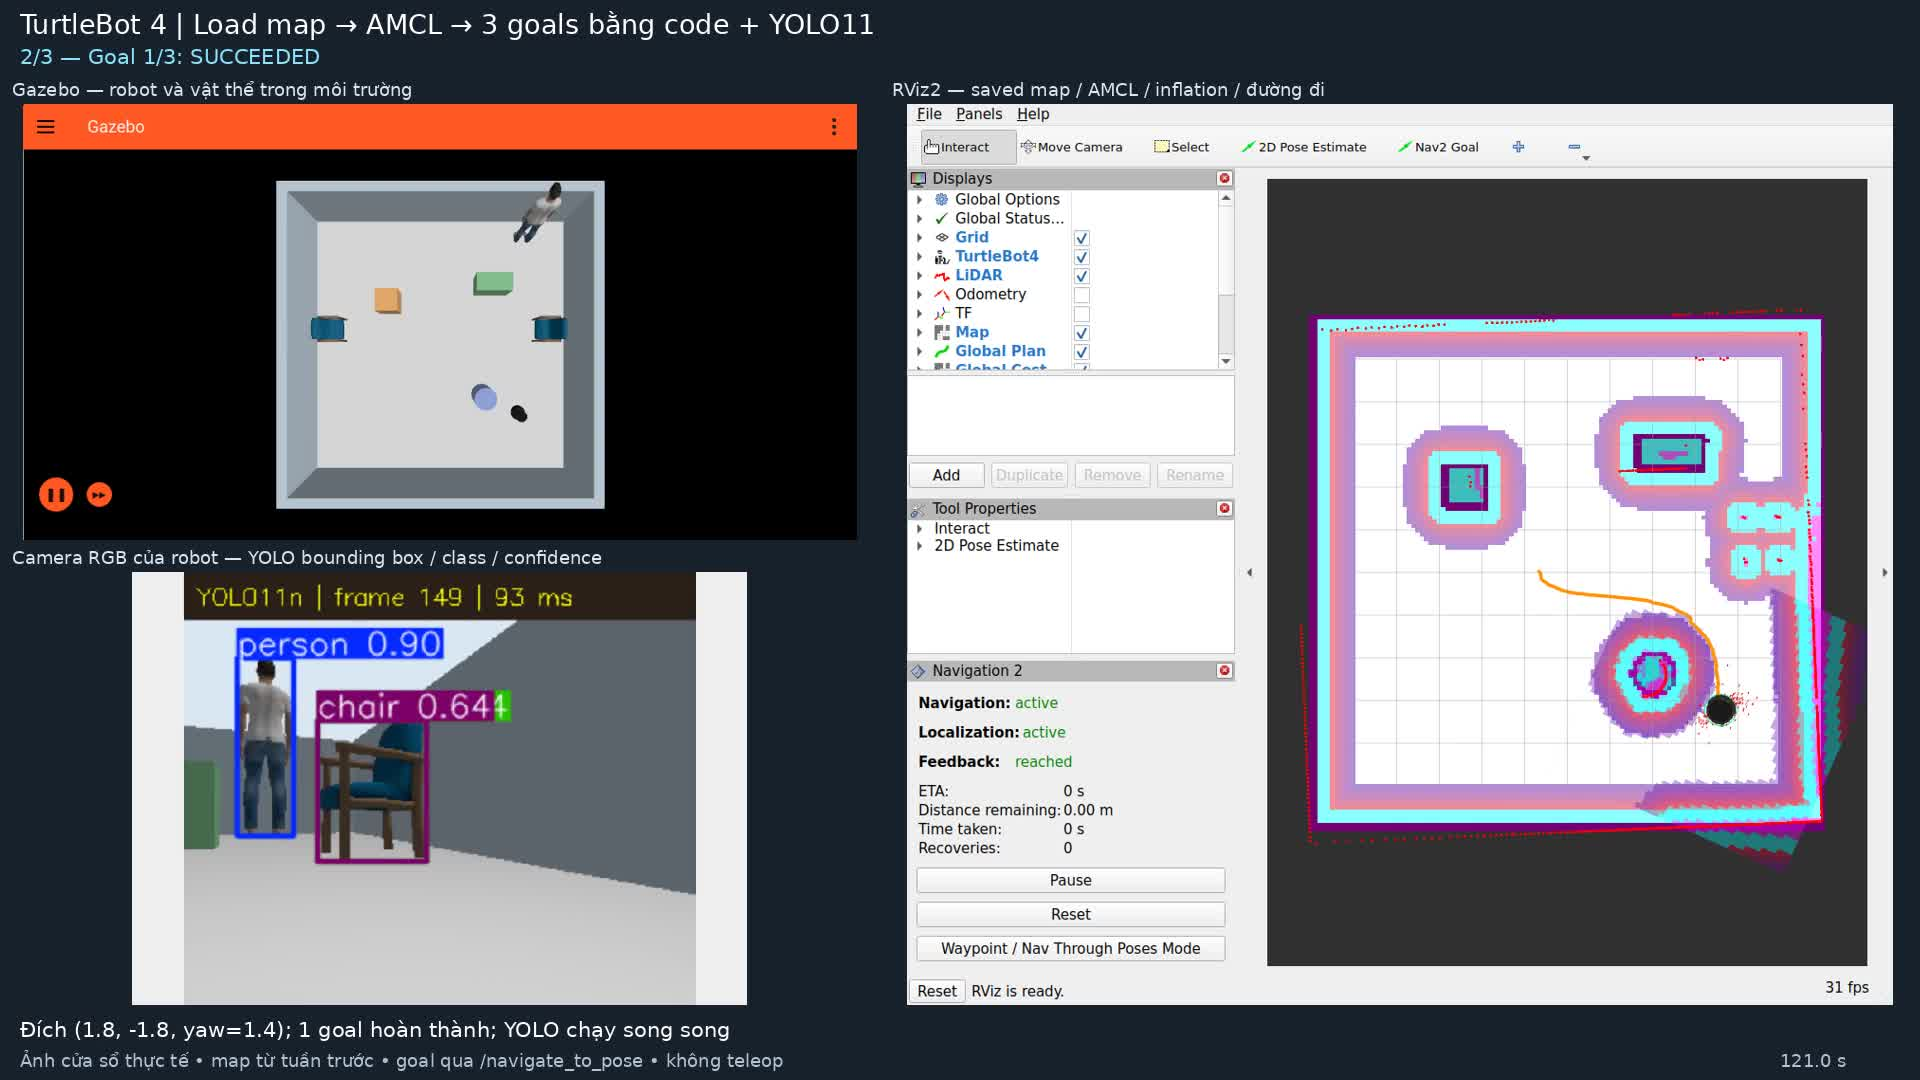
\includegraphics[width=\linewidth,trim=0 0 0 0,clip]{figures/goal1.jpg}\caption{Goal 1 đạt}\end{subfigure}\hfill
\begin{subfigure}[b]{0.32\linewidth}\centering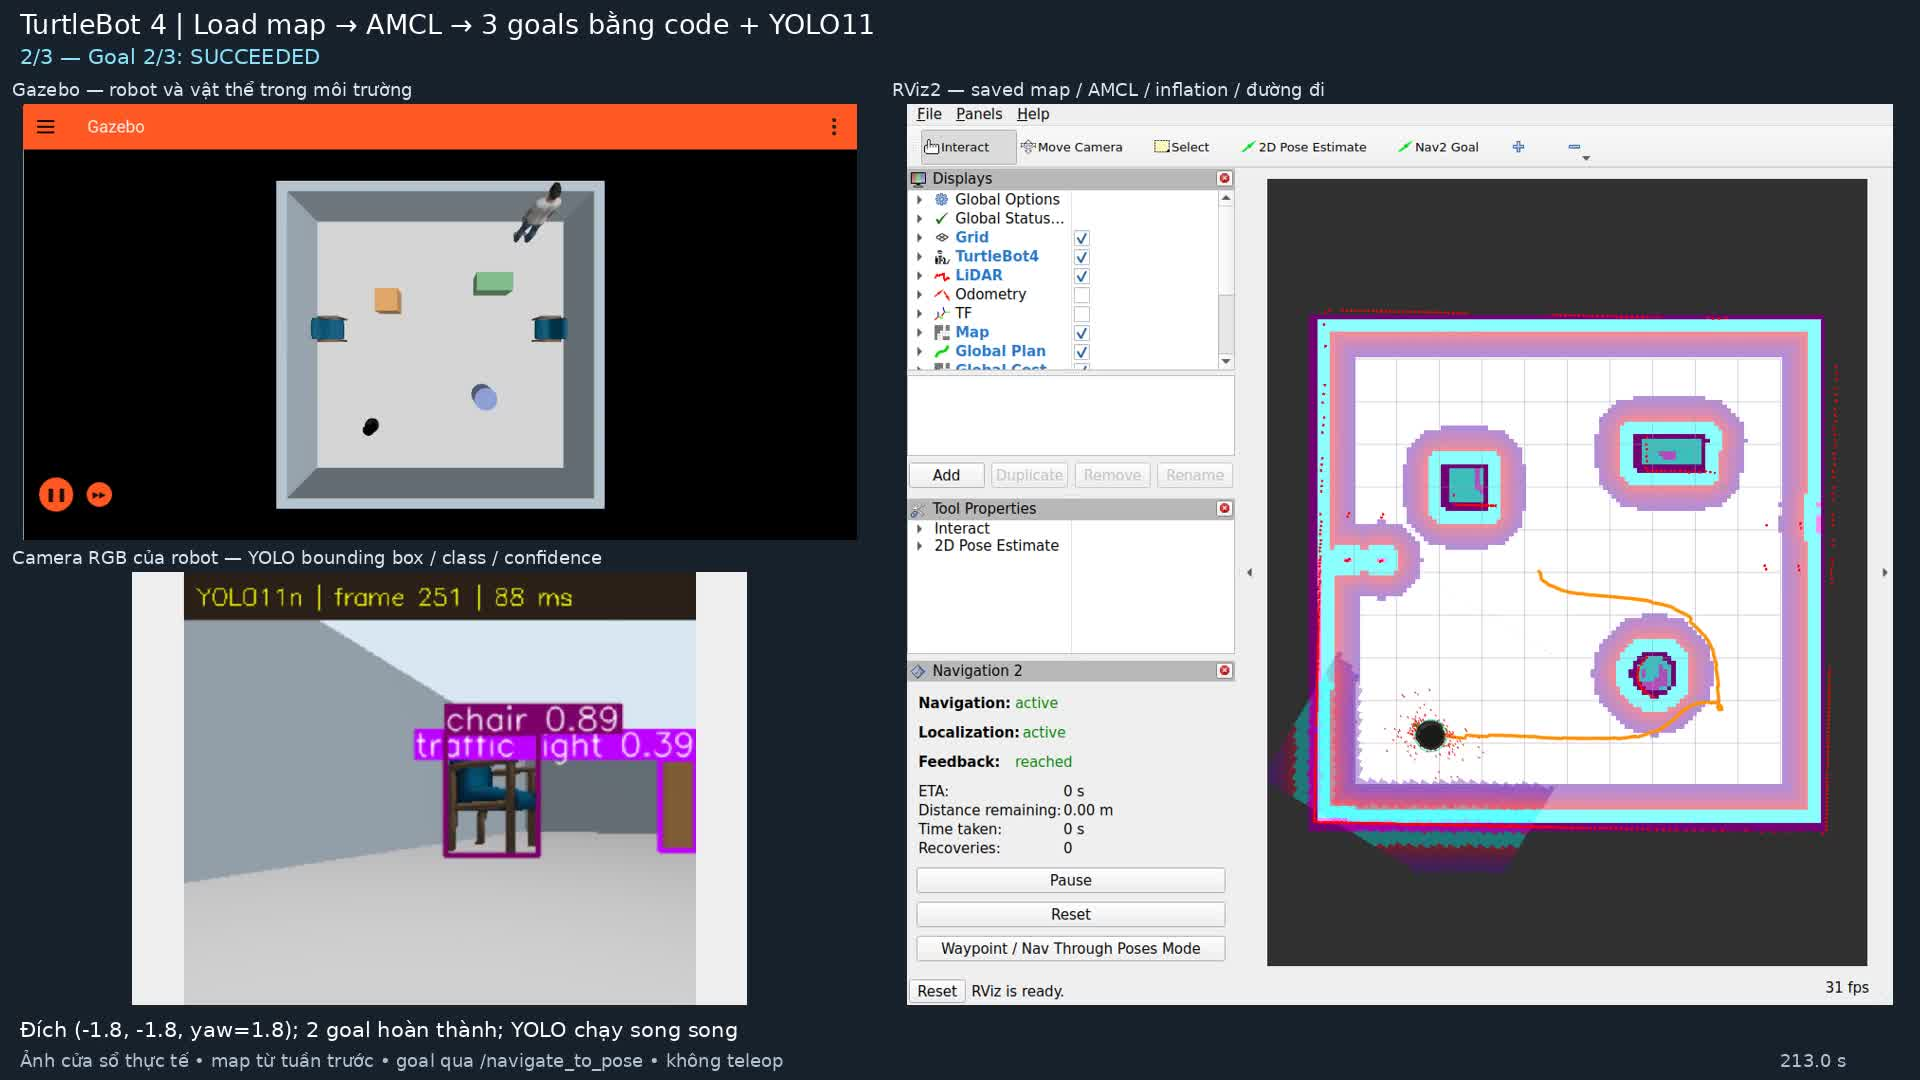
\includegraphics[width=\linewidth]{figures/goal2.jpg}\caption{Goal 2 đạt}\end{subfigure}\hfill
\begin{subfigure}[b]{0.32\linewidth}\centering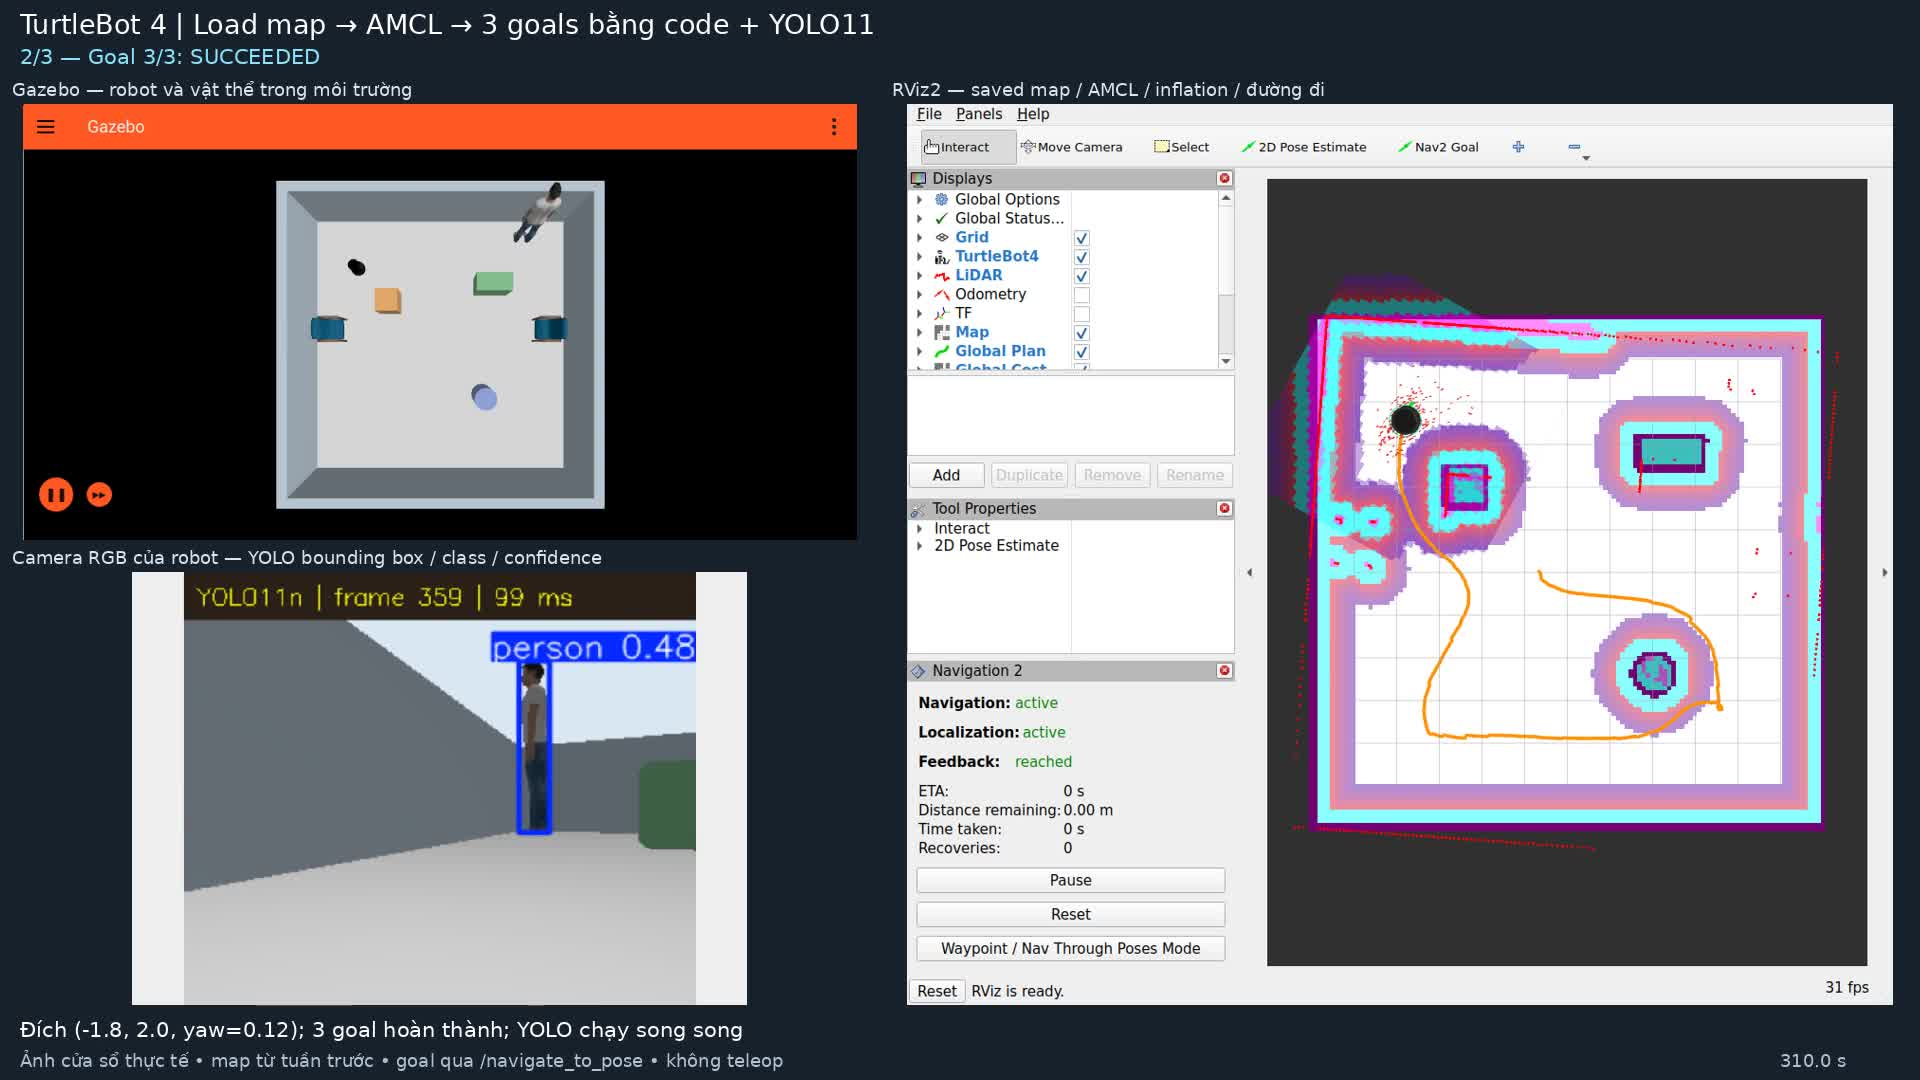
\includegraphics[width=\linewidth]{figures/goal3.jpg}\caption{Goal 3 đạt}\end{subfigure}
\caption{Ảnh chụp từ video tại thời điểm hoàn thành từng goal (Gazebo, camera YOLO, RViz2 với đường đi cam, costmap, \texttt{Feedback: reached}).}\label{fig:three}
\end{figure}

\begin{figure}[htbp]
\centering\figw{0.5}{done_rviz.png}
\caption{RViz2 sau khi đi hết ba goal: bản đồ, global costmap có vùng inflation, đường đi toàn cục (cam), điểm LiDAR (đỏ). \texttt{Navigation: active}, \texttt{Localization: active}, \texttt{Recoveries: 0}.}\label{fig:nav}
\end{figure}

%================== 7. YOLO ==================
\section{Phần 4 -- Nhận diện vật thể bằng YOLO}
\subsection{Node YOLO}
Node \texttt{turtlebot4\_yolo\_camera} (\texttt{scripts/yolo\_camera.py}) dùng mô hình \textbf{YOLO11n} (Ultralytics, trọng số COCO \texttt{yolo11n.pt}) chạy trên CPU với PyTorch~2.5.1. Các bước xử lý mỗi khung hình:
\begin{enumerate}[nosep]
  \item Subscribe \texttt{/oakd/rgb/preview/image\_raw} (QoS \texttt{sensor\_data}); chỉ giữ khung mới nhất để không bị trễ tích lũy.
  \item Timer 5 Hz: chuyển \texttt{sensor\_msgs/Image}$\to$OpenCV (\texttt{bgr8}) bằng \texttt{CvBridge.imgmsg\_to\_cv2}.
  \item \texttt{model.predict(image, imgsz=640, conf=0.3)}.
  \item Vẽ bounding box, tên class, confidence bằng \texttt{result.plot()}, thêm thanh tiêu đề (số khung, thời gian suy luận).
  \item Publish ảnh lên \texttt{/yolo/annotated\_image} (xem được trong RViz2), publish JSON lên \texttt{/yolo/detections}, hiển thị cửa sổ OpenCV (\texttt{--display}), in log ra terminal và lưu \texttt{detections.jsonl}.
\end{enumerate}
\begin{lstlisting}
self.subscription = self.create_subscription(
    Image, args.topic, self.receive, qos_profile_sensor_data)
...
image = self.bridge.imgmsg_to_cv2(message, desired_encoding='bgr8')
result = self.model.predict(image, imgsz=self.args.imgsz,
                            conf=self.args.conf, device='cpu', verbose=False)[0]
for box in result.boxes:
    name = result.names[int(box.cls.item())]
    objects.append({'class': name, 'confidence': float(box.conf.item()),
                    'xyxy': [float(v) for v in box.xyxy[0].tolist()]})
annotated = cv2.copyMakeBorder(result.plot(), 30, 0, 0, 0, cv2.BORDER_CONSTANT, value=(25,32,42))
self.annotated.publish(self.bridge.cv2_to_imgmsg(annotated, encoding='bgr8'))
self.detections.publish(String(data=json.dumps(payload)))
\end{lstlisting}
Thông tin phát hiện được in ra terminal mỗi 2 s, ví dụ:
\begin{lstlisting}[language={},numbers=none]
[turtlebot4_yolo_camera]: YOLO ready: yolo11n.pt; input /oakd/rgb/preview/image_raw
[turtlebot4_yolo_camera]: frame=1: chair 0.90
[turtlebot4_yolo_camera]: frame=161: person 0.93
\end{lstlisting}

\subsection{Kết quả nhận diện}
Trong lần chạy, node nhận 2\,285 khung và xử lý 378 khung (5 Hz), trong đó 199 khung có ít nhất một vật thể; 325 khung xử lý khi robot đang điều hướng, 146 khung trong số đó có phát hiện. Thời gian suy luận $\approx 80$--$110$ ms/khung trên CPU.
\begin{table}[htbp]
\centering\small
\begin{tabular}{lccl}
\toprule
\textbf{Class} & \textbf{Số lần phát hiện} & \textbf{Conf. cao nhất} & \textbf{Nhận xét} \\\midrule
chair & 134 & 0,926 & đúng (2 ghế trong môi trường) \\
person & 77 & 0,929 & đúng (người đứng) \\
bench & 19 & 0,700 & ghế nhìn nghiêng bị gán nhãn trùng \\
traffic light & 10 & 0,575 & nhận nhầm cạnh hộp/tường \\
umbrella & 4 & 0,346 & nhận nhầm góc tường \\\bottomrule
\end{tabular}
\caption{Thống kê phát hiện của YOLO11n (ngưỡng conf $=0{,}3$).}
\end{table}
Hai class chính xác là \emph{chair} và \emph{person}. Ba class còn lại có độ tin cậy thấp hơn và thực chất là nhận nhầm (Hình~\ref{fig:fp}); nguyên nhân là mô hình COCO được huấn luyện trên ảnh thật, trong khi mô phỏng chỉ có các khối hình học đơn giản. Có thể giảm nhầm lẫn bằng cách tăng ngưỡng \texttt{--conf} lên $0{,}5$ hoặc dùng YOLO-World với tập class giới hạn.

\begin{figure}[htbp]
\centering
\begin{subfigure}[b]{0.31\linewidth}\centering\figw{1}{yolo_chair.jpg}\caption{chair 0,93}\end{subfigure}\hfill
\begin{subfigure}[b]{0.31\linewidth}\centering\figw{1}{yolo_person.jpg}\caption{person 0,93}\end{subfigure}\hfill
\begin{subfigure}[b]{0.31\linewidth}\centering\figw{1}{done_cam.png}\caption{Cửa sổ OpenCV khi chạy}\end{subfigure}
\caption{Kết quả nhận diện đúng: bounding box, tên class, độ tin cậy.}\label{fig:yolo}
\end{figure}
\begin{figure}[htbp]
\centering\figw{0.75}{yolo_fp.png}
\caption{Các phát hiện kém tin cậy (trái$\to$phải): bench 0,72 (cùng chiếc ghế), umbrella 0,35 (góc tường), traffic light 0,58 (cạnh hộp).}\label{fig:fp}
\end{figure}

%================== 8. CHẠY ==================
\section{Hướng dẫn cài đặt và chạy}
\begin{lstlisting}[language=bash,numbers=none]
git clone -b turtlebot https://github.com/TranThang27/UR3_drawing.git
cd UR3_drawing/turtlebot
sudo apt install ros-humble-turtlebot4-simulator ros-humble-turtlebot4-navigation \
  ros-humble-slam-toolbox ros-humble-nav2-bringup ros-humble-cv-bridge \
  ros-humble-rmw-cyclonedds-cpp ros-humble-rviz2 ffmpeg wmctrl
./run.sh setup && ./run.sh doctor     # tai runtime, kiem tra package
./run.sh setup-yolo                   # torch CPU + ultralytics + yolo11n.pt

# Cach 1: tu dong toan bo (load map -> AMCL -> 3 goal bang code -> YOLO -> quay video)
./run.sh yolo-demo --output reports/nav_yolo_demo_new

# Cach 2: tung buoc
./run.sh sim rviz_config:="$PWD/config/localization.rviz"     # terminal 1
./run.sh undock; ./run.sh remove-dock                         # terminal 2
./run.sh localize maps/map.yaml                               # terminal 3 (AMCL)
./run.sh nav2                                                 # terminal 4 (Nav2)
./run.sh yolo --display                                       # terminal 5 (YOLO)
./run.sh goals --goals-file config/goals.yaml --dwell 6       # terminal 6 (3 goal)
\end{lstlisting}

%================== 9. KẾT LUẬN ==================
\section{Nhận xét và kết luận}
\paragraph{Kết quả đạt được.} Đã nạp lại bản đồ cũ và định vị thành công bằng AMCL (sai lệch $0{,}019$ m); robot tự đi qua 3 goal liên tiếp bằng node Python gọi action \texttt{/navigate\_to\_pose}, không va chạm, không can thiệp thủ công; node YOLO11n chạy song song, nhận đúng ghế và người với độ tin cậy trên $0{,}9$ và publish kết quả lên \texttt{/yolo/annotated\_image}.

\paragraph{Hạn chế.}
\begin{itemize}[nosep]
  \item Sai số yaw tại goal $\approx 0{,}25$ rad do dung sai mặc định của Nav2; có thể giảm bằng cách siết \texttt{yaw\_goal\_tolerance} trong \texttt{nav2.yaml}.
  \item YOLO chạy trên CPU ($\sim 10$ FPS lý thuyết, cấu hình 5 Hz); có nhận nhầm class với các khối hình học đơn giản.
  \item Initial pose cần biết trước vị trí xuất phát; nếu không biết, có thể dùng \texttt{/reinitialize\_global\_localization} của AMCL.
  \item Mỗi goal mất khoảng 85--90 s vì robot chạy chậm và Gazebo chạy trên CPU/GPU tích hợp.
\end{itemize}
\paragraph{Hướng phát triển.} Gắn vị trí vật thể phát hiện vào bản đồ bằng ảnh depth của OAK-D; dùng \texttt{nav2\_waypoint\_follower} để đi qua nhiều điểm không dừng; thay YOLO11n bằng YOLO-World để nhận diện theo từ khóa.

\section*{Liên kết}
\begin{itemize}[nosep]
  \item Video demo (Google Drive): \url{https://drive.google.com/drive/folders/1LF-GkSyY50TnkUzGGbq_RCvAMGTMZOS7?hl=vi}
  \item GitHub (nhánh \texttt{turtlebot}, thư mục \texttt{turtlebot/}): \url{https://github.com/TranThang27/UR3_drawing/tree/turtlebot/turtlebot}
\end{itemize}

\end{document}
